% Standalone version of the baseline vs reverse-mode comparison chart.
% This is the same chart that appears in the thesis Chapter 5.
%
% To compile standalone (requires pgfplots package):
%   pdflatex baseline_vs_reverse_before_after.tex
%
% Data: median of 5 runs, single-threaded with PRAGMA threads=1, on the
% optimised release build of DuckDB.
%   - "before" = original row-by-row reverse-mode AD
%   - "after"  = tiled vectorisation (tile size 256, operation-outer inner loop)

\documentclass[12pt]{article}
\usepackage[a4paper,margin=2cm,landscape]{geometry}
\usepackage{pgfplots}
\pgfplotsset{compat=1.17}
\pagestyle{empty}

\begin{document}
\noindent
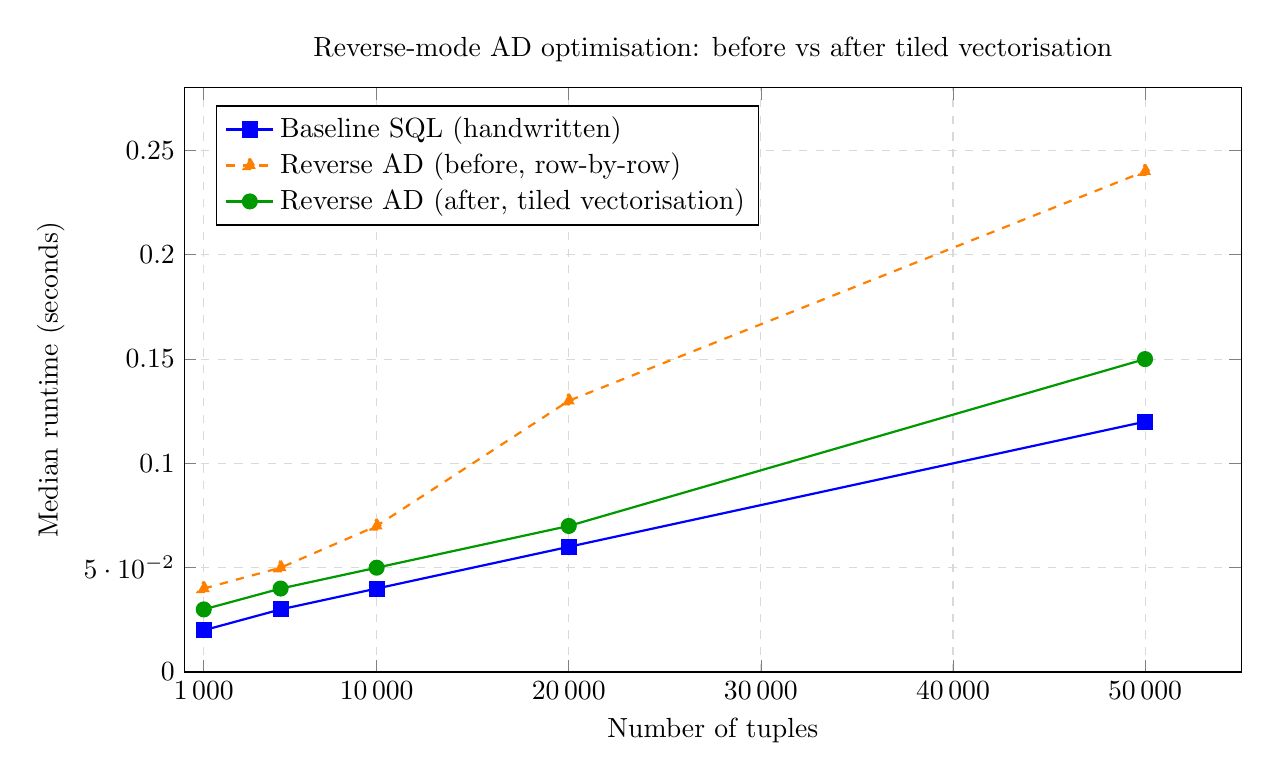
\begin{tikzpicture}
\begin{axis}[
    width=15cm,
    height=9cm,
    title={Reverse-mode AD optimisation: before vs after tiled vectorisation},
    xlabel={Number of tuples},
    ylabel={Median runtime (seconds)},
    xmin=0, xmax=55000,
    ymin=0, ymax=0.28,
    xtick={1000,10000,20000,30000,40000,50000},
    scaled x ticks=false,
    xticklabel style={/pgf/number format/1000 sep=\,},
    legend pos=north west,
    legend cell align=left,
    grid=major,
    grid style={dashed,gray!30},
]

% Baseline (unchanged, both before and after)
\addplot[color=blue, mark=square*, thick, mark size=2.5pt] coordinates {
    (1000, 0.02)
    (5000, 0.03)
    (10000, 0.04)
    (20000, 0.06)
    (50000, 0.12)
};
\addlegendentry{Baseline SQL (handwritten)}

% Reverse AD before optimisation
\addplot[color=orange, mark=triangle*, thick, dashed, mark size=2.5pt] coordinates {
    (1000, 0.04)
    (5000, 0.05)
    (10000, 0.07)
    (20000, 0.13)
    (50000, 0.24)
};
\addlegendentry{Reverse AD (before, row-by-row)}

% Reverse AD after optimisation
\addplot[color=green!60!black, mark=*, thick, mark size=2.5pt] coordinates {
    (1000, 0.03)
    (5000, 0.04)
    (10000, 0.05)
    (20000, 0.07)
    (50000, 0.15)
};
\addlegendentry{Reverse AD (after, tiled vectorisation)}

\end{axis}
\end{tikzpicture}
\end{document}
